\usetikzlibrary{arrows.meta,shapes.multipart,patterns}

\tikzset{
    stackBox/.style={very thick},
    onStack/.style={thick},
    frameOne/.style={fill=blue!15},
    frameTwo/.style={fill=red!15},
    markLine/.style={blue!50!black},
    markLineB/.style={red!90!black},
    hiLine/.style={red!90!black},
}

\begin{frame}{malloc/new guard pages}
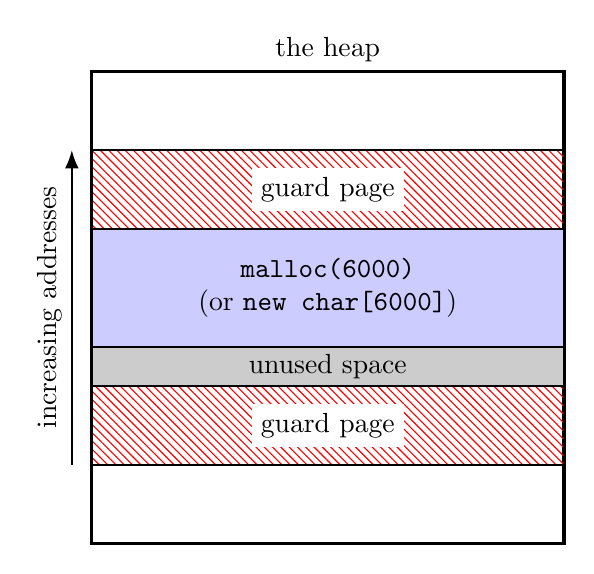
\begin{tikzpicture}
    \draw[thick,-Latex] (-0.25,-5) -- (-0.25, -1) node [midway, above, sloped] {increasing addresses};
    \node[anchor=south] at (3, 0) {the heap};
    \draw[stackBox] (0, 0) rectangle (6, -6);
    \draw[onStack,fill=blue!20] (0, -2) rectangle (6, -3.5)
        node[midway,align=center] {\texttt{malloc(6000)} \\ (or \texttt{new char[6000]}) };
    \draw[onStack,pattern=north west lines,pattern color=red] (0, -1) rectangle (6, -2)
        node[midway,fill=white] {guard page};
    \draw[onStack,pattern=north west lines,pattern color=red] (0, -4) rectangle (6, -5)
        node[midway,fill=white] {guard page};
    \draw[onStack,fill=black!20] (0, -3.5) rectangle (6, -4)
        node[midway] {unused space};
\end{tikzpicture}
\end{frame}

\begin{frame}{guard pages}
    \begin{itemize}
    \item deliberate holes
    \item accessing --- segfualt
    \item call to OS to allocate (not very fast)
    \item likely to `waste' memory
        \begin{itemize}
        \item guard around object? minimum 4KB object
        \end{itemize}
    \end{itemize}
\end{frame}

\begin{frame}{guard pages for malloc/new}
    \begin{itemize}
    \item can implement malloc/new by placing guard pages around allocations
        \begin{itemize}
        \item commonly done by real malloc/new's for \myemph{large allocations}
        \end{itemize}
    \item problem: minimum actual allocation 4KB
    \item problem: substantially slower
    \item example: ``Electric Fence'' allocator for Linux (early 1990s)
    \end{itemize}
\end{frame}


\begin{frame}[fragile,label=stackGuard]{stack canary alternative}
\begin{tikzpicture}
\draw[stackBox] (0, 0) rectangle (6, -6);
\draw[thick,-Latex] (-.25,-5) -- (-.25, -1) node [midway, above, sloped] {increasing addresses};
\node[at={(4, 0.1)},anchor=south] { highest address (stack started here)};
\node[at={(4, -6.1)},anchor=north] { lowest address (stack grows here)};

\draw[onStack] (0, -.25) rectangle (6, -1.25) node[midway,align=center,font=\small] (stackAddr)
     {return address for {\tt vulnerable}: \\
     {\fontsize{10}{11}\selectfont\tt\color{black}0x40fd37}
     };
    \draw[onStack,pattern=north west lines,pattern color=red] (0, -1.25) rectangle (6, -3.25) node[midway,align=center,font=\small,fill=white] {``guard page'' \\ minimum 4KB};
\draw[onStack,fill=blue!20] (0, -3.25) rectangle (6, -4.25) node[midway,align=center,font=\small] {buffer};
\begin{visibleenv}<2->
\draw[black,Latex-] (6.1, -1.25) -- ++(.5cm, 0cm) node[right,font=\small\tt] {0x7FFFF 2000};
\draw[black,Latex-] (6.1, -3.25) -- ++(.5cm, 0cm) node[right,font=\small\tt] {0x7FFFF 1000};

\matrix[tight matrix,overlay,
    column 1/.style={nodes={text width=2.25cm,minimum height=1cm,font=\fontsize{9}{10}\selectfont\tt}},
    column 2/.style={nodes={minimum height=1cm}},
    column 3/.style={nodes={minimum height=1cm}},
    ] at (12.4, -2) {
        address \& read \& write \\
    0x7FFFF2000- 0x7FFFF2FFF \& yes \& yes \\
    0x7FFFF1000- 0x7FFFF1FFF \& no \& no \\
    0x7FFFF0000- 0x7FFFF0FFF \& yes \& yes \\
};
\end{visibleenv};

\end{tikzpicture}
\end{frame}

\begin{frame}[fragile,label=stackGuardB]{stack canary alternative 2}
\begin{tikzpicture}
\draw[stackBox] (0, 0) rectangle (6, -6);
\draw[thick,-Latex] (-.25,-5) -- (-.25, -1) node [midway, above, sloped] {increasing addresses};
\node[at={(4, 0.1)},anchor=south] { highest address (stack started here)};
\node[at={(4, -6.1)},anchor=north] { lowest address (stack grows here)};

\draw[onStack] (0, -.25) rectangle (6, -1.25) node[midway,align=center,font=\small] (stackAddr)
     {return address for {\tt vulnerable}: \\
     {\fontsize{10}{11}\selectfont\tt\color{black}0x40fd37}
     };
\draw[onStack,pattern=north west lines,pattern color=black!50] (0, -1.25) rectangle (6, -2.25) node[midway,align=center,font=\small,fill=white] {unused space};
\draw[onStack,fill=blue!20] (0, -2.25) rectangle (6, -4.25) node[midway,align=center,font=\small] {buffer};
\begin{visibleenv}<2->
\draw[black,Latex-] (6.1, -.25) -- ++(.5cm, 0cm) node[right,font=\small\tt] {0x7FFFF 2000};
\draw[black,Latex-] (6.1, -2.25) -- ++(.5cm, 0cm) node[right,font=\small\tt] {0x7FFFF 1000};

\matrix[tight matrix,
    column 1/.style={nodes={text width=2.25cm,minimum height=1cm,font=\fontsize{9}{10}\selectfont\tt}},
    column 2/.style={nodes={minimum height=1cm}},
    column 3/.style={nodes={minimum height=1cm}},
    ] at (12.3, -1) {
        address \& read \& write\\
    0x7FFFF2000- 0x7FFFF2FFF \& yes \& yes \\
    0x7FFFF1000- 0x7FFFF1FFF \& yes \& \myemph<2>{no} \\
    0x7FFFF0000- 0x7FFFF0FFF \& yes \& yes \\
};
\end{visibleenv};

\end{tikzpicture}
\end{frame}

